\chapter{Hàm sóng, ma trận mật độ và tính địa phương}

\lectureoverview{Định lý Bell được hoãn lại vì một lý do cốt yếu: trước khi hỏi Bell cấm điều gì, ta phải nói chính xác vướng víu là gì. Một trạng thái hai phần là vướng víu khi nó không thể được phân tích thành một trạng thái cho Alice và một trạng thái cho Bob. Các hàm sóng làm cho tiêu chuẩn đó trở nên cụ thể, các tương quan bộc lộ các hệ quả của nó, và trạng thái singlet cung cấp ví dụ quyết định. Khi đó ma trận mật độ rút gọn trở thành mô tả địa phương đầy đủ của một phần trong một toàn thể vướng víu. Với bộ công cụ đó trong tay, phép đo xuất hiện như một tương tác gây vướng víu, ranh giới hệ--người quan sát có thể được dời đi mà không làm thay đổi các dự đoán, và sự căng thẳng bề ngoài giữa vướng víu và tính địa phương có thể được phát biểu một cách sắc nét: các lựa chọn ở xa làm thay đổi các tương quan có điều kiện, nhưng không làm thay đổi các thống kê vô điều kiện có thể dùng để truyền tín hiệu.}

\section{Vướng víu thực sự có nghĩa là gì}

Rất dễ muốn đi thẳng đến định lý Bell. Định lý ấy rất đẹp, nhưng ý nghĩa của nó không thể tách rời khỏi cấu trúc mà nó kiểm định. Vì vậy, câu hỏi cấp thiết hơn lúc này chưa phải là liệu cơ học lượng tử có vi phạm một bất đẳng thức Bell hay không, mà là một trạng thái vướng víu nói gì về một hệ hợp thành.

Một cụm từ thường gặp là hai hệ vướng víu \emph{cùng chia sẻ một trạng thái}. Cụm từ ấy không phân biệt được điều gì cả. Mọi hệ hợp thành đều có một trạng thái, dù có vướng víu hay không. Sự phân biệt nằm ở tính phân tích thành thừa số. Nếu \(A\) và \(B\) có các không gian Hilbert \(\mathcal H_A\) và \(\mathcal H_B\), thì trạng thái của cặp nằm trong
\begin{equation}
\mathcal H_{AB}=\mathcal H_A\otimes\mathcal H_B.
\end{equation}
Một trạng thái thuần túy là trạng thái tích khi nó có thể được viết
\begin{equation}
\ket{\Psi}_{AB}=\ket{\psi}_A\otimes\ket{\phi}_B.
\label{eq:l7-product-state}
\end{equation}
Nếu không tồn tại cặp thừa số nào như vậy, thì \(\ket{\Psi}_{AB}\) là vướng víu.

\begin{classroomqa}
\audiencequestion{Có phải vướng víu đơn giản chỉ có nghĩa là cả hai hệ cùng xuất hiện trong một vectơ trạng thái không?}
\lecturerresponse{Không. Một trạng thái tích cũng thuộc không gian Hilbert của toàn bộ cặp. Vướng víu là phát biểu mạnh hơn, độc lập với cơ sở, rằng vectơ của toàn bộ không thể được viết thành một vectơ cho Alice nhân với một vectơ cho Bob.}
\end{classroomqa}

\begin{classroomqa}
\audiencequestion{Liệu một phép đổi cơ sở khéo léo có thể biến một trạng thái vướng víu thành một trạng thái tích không?}
\lecturerresponse{Không, nếu phép đổi cơ sở là địa phương, nghĩa là một phép đổi cơ sở cho Alice và một phép khác cho Bob. Các phép đổi cơ sở địa phương làm thay đổi các tọa độ của từng thừa số nhưng không làm thay đổi việc trạng thái có phân tích thành thừa số hay không. Một cơ sở hoàn toàn tùy ý của không gian Hilbert chung có thể che giấu cấu trúc tích tensor, nhưng nó không làm thay đổi những bậc tự do vật lý nào thuộc về Alice và Bob.}
\end{classroomqa}

\section{Hàm sóng như các tọa độ trong không gian Hilbert}

Từ \emph{hàm sóng} gợi lên một hình ảnh lịch sử không thuộc về định nghĩa toán học của nó. Hàm sóng là biểu diễn tọa độ của một vectơ trạng thái trong một cơ sở được chọn. Hãy cho một tập đầy đủ các đại lượng quan sát giao hoán có các vectơ riêng đồng thời
\begin{equation}
\ket{a,b,c,\ldots}.
\end{equation}
Các nhãn phải là đầy đủ: khi được xét cùng nhau, chúng phân biệt mọi vectơ trong cơ sở. Khi đó
\begin{align}
\ket{\Psi}
&=\sum_{a,b,c,\ldots}
\ket{a,b,c,\ldots}
\braket{a,b,c,\ldots}{\Psi} \\
&=\sum_{a,b,c,\ldots}
\psi(a,b,c,\ldots)\ket{a,b,c,\ldots},
\label{eq:l7-wavefunction-expansion}
\end{align}
trong đó
\begin{equation}
\psi(a,b,c,\ldots)
=\braket{a,b,c,\ldots}{\Psi}.
\label{eq:l7-wavefunction-definition}
\end{equation}
Đối với các nhãn liên tục, các tổng tương ứng trở thành các tích phân.

\begin{figure}[htbp]
\centering
\includegraphics[width=0.88\textwidth]{lecture_07_figure_01.png}
\caption{Hàm sóng như tập hợp các hệ số của một trạng thái trong một cơ sở đầy đủ.}
\lectureframe{00:07:00}
\end{figure}

Đối với một hạt trong không gian ba chiều, các nhãn giao hoán có thể là \(x,y,z\), và
\begin{equation}
\psi(x,y,z)=\braket{x,y,z}{\Psi}
\end{equation}
là hàm sóng trong không gian vị trí quen thuộc của Schr\"odinger. Đối với một spin trong cơ sở \(\sigma_z\), hàm sóng chỉ đơn giản là cặp
\begin{equation}
\psi(u)=\braket{u}{\Psi},
\qquad
\psi(d)=\braket{d}{\Psi}.
\end{equation}
Đối với hai spin, cần hai nhãn:
\begin{equation}
\Psi(a,b)=\braket{a,b}{\Psi},
\qquad
a,b\in\{u,d\}.
\label{eq:l7-two-spin-wavefunction}
\end{equation}
Không có gì trong định nghĩa này đòi hỏi phải có một sóng theo nghĩa đen trong không gian.

\begin{classroomqa}
\audiencequestion{Việc đổi cơ sở của hàm sóng có phải là một phép biến đổi Fourier không?}
\lecturerresponse{Phép biến đổi Fourier là phép đổi cơ sở cụ thể giữa biểu diễn vị trí và biểu diễn xung lượng. Tổng quát hơn, mọi phép đổi cơ sở trực chuẩn đều là một phép biến đổi unita của các tọa độ. Việc chuyển từ cơ sở \(\sigma_z\) sang cơ sở \(\sigma_x\) là tương tự một phép biến đổi Fourier, dù đó là một ma trận unita hữu hạn chiều chứ không phải phép biến đổi tích phân vị trí--xung lượng.}
\end{classroomqa}

\begin{classroomqa}
\audiencequestion{Nếu hàm sóng thay đổi dưới một phép đổi cơ sở, thì trạng thái vật lý có thay đổi không?}
\lecturerresponse{Không. Ket \(\ket{\Psi}\) là trạng thái trừu tượng. Các số \(\psi(a,b,c,\ldots)\) là các tọa độ của nó trong một cơ sở đã chọn. Việc đổi tọa độ làm thay đổi các số ấy trong khi vectơ và mọi dự đoán vật lý vẫn không đổi.}
\end{classroomqa}

\section{Giá trị kỳ vọng theo các thành phần}

Trước khi đưa vào ma trận mật độ, hãy làm rõ cấu trúc thành phần của một giá trị kỳ vọng. Gọi \(L\) là một đại lượng quan sát, với các phần tử ma trận
\begin{equation}
L_{a'a}=\bra{a'}L\ket{a}.
\label{eq:l7-matrix-elements}
\end{equation}
Nếu \(\ket{\Psi}=\sum_a\psi(a)\ket{a}\), thì
\begin{align}
\expect{L}
&=\bra{\Psi}L\ket{\Psi} \\
&=\sum_{a',a}
\psi^*(a')\bra{a'}L\ket{a}\psi(a) \\
&=\sum_{a',a}\psi^*(a')L_{a'a}\psi(a).
\label{eq:l7-expectation-components}
\end{align}

\begin{figure}[htbp]
\centering
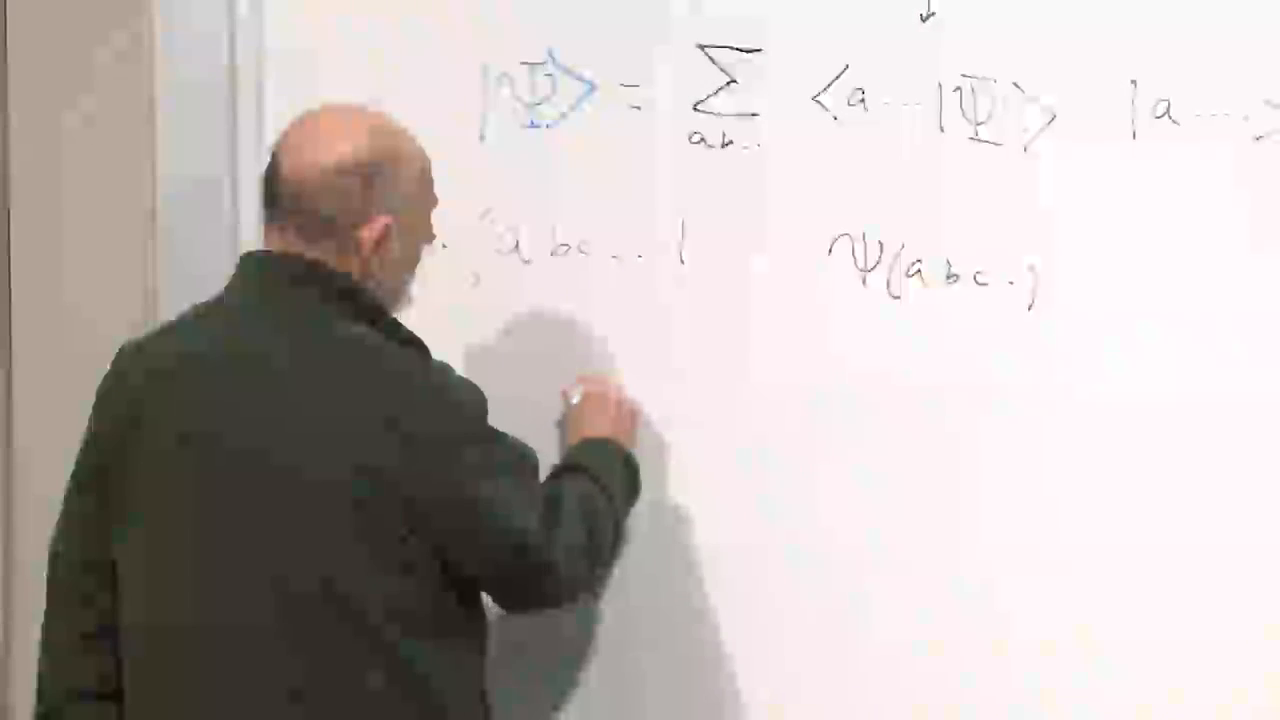
\includegraphics[width=0.88\textwidth]{lecture_07_figure_02.png}
\caption{Biểu thức kẹp của giá trị kỳ vọng được khai triển theo các hệ số hàm sóng và các phần tử ma trận.}
\lectureframe{00:14:08}
\end{figure}

Bây giờ hãy chia hệ thành phần của Alice và phần của Bob. Gọi \(a\) là một nhãn cơ sở đầy đủ cho Alice và \(b\) là một nhãn như vậy cho Bob:
\begin{equation}
\ket{\Psi}_{AB}
=\sum_{a,b}\Psi(a,b)\ket{a,b}.
\label{eq:l7-composite-expansion}
\end{equation}
Một đại lượng quan sát chỉ thuộc về Alice được biểu diễn trên không gian hợp thành bởi
\begin{equation}
L_A=L\otimes I_B,
\end{equation}
nên các phần tử ma trận của nó là
\begin{equation}
\bra{a',b'}L_A\ket{a,b}
=L_{a'a}\delta_{b'b}.
\label{eq:l7-alice-local-matrix}
\end{equation}
Tương tự, một đại lượng quan sát địa phương đối với Bob có dạng
\begin{equation}
M_B=I_A\otimes M,
\qquad
\bra{a',b'}M_B\ket{a,b}
=\delta_{a'a}M_{b'b}.
\label{eq:l7-bob-local-matrix}
\end{equation}
Toán tử đơn vị trên thừa số không bị tác động là phát biểu toán học cho việc phép tác động của Alice chỉ tác động lên Alice và phép tác động của Bob chỉ tác động lên Bob.

Thay Phương trình~\eqref{eq:l7-alice-local-matrix} vào giá trị kỳ vọng, ta được
\begin{equation}
\expect{L_A}
=\sum_{a',a,b}
\Psi^*(a',b)L_{a'a}\Psi(a,b).
\label{eq:l7-local-expectation}
\end{equation}
Công thức này đã chứa ma trận mật độ rút gọn; ta sẽ sắp xếp lại nó sau khi trước hết xem sự phân tích thành thừa số dẫn đến điều gì.

\begin{classroomqa}
\audiencequestion{Vì sao trong Phương trình~\eqref{eq:l7-local-expectation} chỉ còn lại một chỉ số của Bob?}
\lecturerresponse{Toán tử đơn vị trên không gian của Bob đóng góp \(\delta_{b'b}\). Nó đặt các nhãn bra và ket ở phía Bob bằng nhau, nên tổng kép theo \(b',b\) rút xuống còn một tổng theo \(b\).}
\end{classroomqa}

\begin{classroomqa}
\audiencequestion{Alice có cần biết Bob dùng cơ sở nào không?}
\lecturerresponse{Không dự đoán vật lý nào phụ thuộc vào cơ sở của Bob. Tổng trên một cơ sở đầy đủ của Bob là một phân giải của toán tử đơn vị. Một cơ sở khác của Bob làm thay đổi các thành phần riêng lẻ \(\Psi(a,b)\), nhưng không làm thay đổi giá trị kỳ vọng của Alice.}
\end{classroomqa}

\section{Trạng thái tích và các tương quan}

Trong một trạng thái tích, hàm sóng chung phân tích thành thừa số:
\begin{equation}
\Psi(a,b)=\psi_A(a)\phi_B(b).
\label{eq:l7-wavefunction-factorization}
\end{equation}
Thay biểu thức này vào Phương trình~\eqref{eq:l7-local-expectation}:
\begin{align}
\expect{L_A}
&=\sum_{a',a,b}
\psi_A^*(a')\phi_B^*(b)
L_{a'a}
\psi_A(a)\phi_B(b) \\
&=\left[
\sum_{a',a}\psi_A^*(a')L_{a'a}\psi_A(a)
\right]
\left[
\sum_b|\phi_B(b)|^2
\right] \\
&=\bra{\psi_A}L\ket{\psi_A}.
\label{eq:l7-product-local-expectation}
\end{align}
Điều kiện chuẩn hóa của Bob làm cho thừa số tương ứng bằng một. Vì thế Alice có đúng cùng các thống kê địa phương như khi hệ của Bob chưa hề được đưa vào.

\begin{figure}[htbp]
\centering
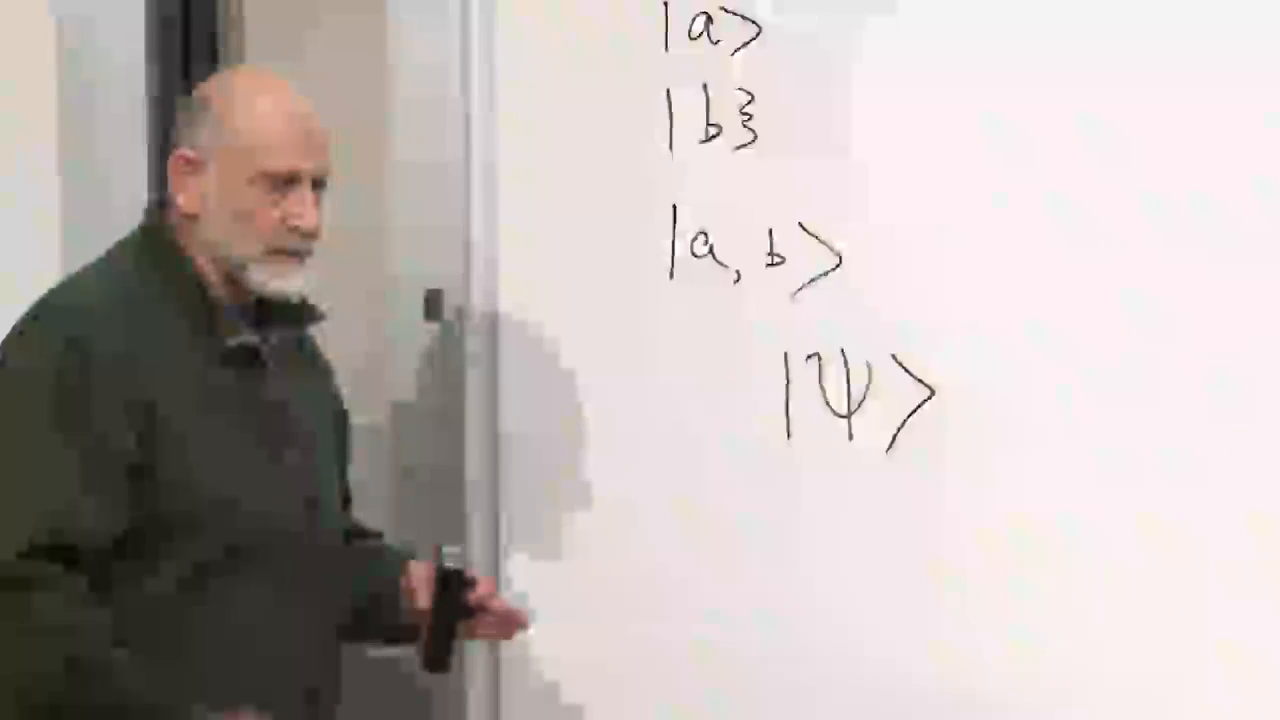
\includegraphics[width=0.88\textwidth]{lecture_07_figure_03.png}
\caption{Sự phân tích thành thừa số của hàm sóng chung và sự tách tương ứng của các giá trị kỳ vọng địa phương.}
\lectureframe{00:29:18}
\end{figure}

Tích của một đại lượng quan sát của Alice với một đại lượng quan sát của Bob có các phần tử ma trận
\begin{equation}
\bra{a',b'}L_A M_B\ket{a,b}
=L_{a'a}M_{b'b}.
\end{equation}
Đối với một trạng thái tích, giá trị kỳ vọng của nó tách ra:
\begin{equation}
\expect{L_A M_B}
=\expect{L_A}\expect{M_B}.
\label{eq:l7-product-correlation-factorization}
\end{equation}
Vì vậy, thật tự nhiên khi định nghĩa tương quan liên thông
\begin{equation}
C(L,M)
=\expect{L_A M_B}
-\expect{L_A}\expect{M_B}.
\label{eq:l7-connected-correlation}
\end{equation}
Mọi trạng thái tích đều có \(C(L,M)=0\) đối với mọi cặp đại lượng quan sát địa phương. Ngược lại, đối với một trạng thái thuần túy hai phần, vướng víu bảo đảm rằng tồn tại một cặp đại lượng quan sát địa phương có tương quan liên thông khác không.

\begin{classroomqa}
\audiencequestion{Liệu \(L_A M_B\) có nghĩa là Bob được đo trước và Alice đo sau không?}
\lecturerresponse{Không. Các toán tử tác dụng lên các vectơ trạng thái; các thiết bị mới thực hiện phép đo. Tích đó có nghĩa là \(M_B\) tác dụng rồi đến \(L_A\) tác dụng. Vì các toán tử nằm trên những thừa số tensor khác nhau, \([L_A,M_B]=0\), nên thứ tự toán học của chúng là không quan trọng. Quy trình thí nghiệm để ước lượng giá trị kỳ vọng chung là một vấn đề riêng.}
\end{classroomqa}

\begin{classroomqa}
\audiencequestion{Trạng thái có thể vẫn vướng víu ngay cả khi một tương quan được chọn triệt tiêu không?}
\lecturerresponse{Chắc chắn có thể. Việc \(C(L,M)\) triệt tiêu chỉ nói rằng cặp đại lượng quan sát cụ thể này không tương quan. Để xác lập sự phân tích thành thừa số cho một trạng thái thuần túy, mọi tương quan chéo địa phương đều phải phân tích thành thừa số. Tương quan một phần cũng không nhất thiết có nghĩa là vướng víu một phần theo bất kỳ nghĩa đơn giản nào bằng một con số; toàn bộ phổ của mật độ rút gọn mới mang thông tin đó.}
\end{classroomqa}

\begin{classroomqa}
\audiencequestion{Mọi trạng thái có tương quan đều là vướng víu sao?}
\lecturerresponse{Đối với các trạng thái thuần túy đang xét, các tương quan không phân tích được thành thừa số bộc lộ vướng víu. Đối với các trạng thái hỗn hợp, các tương quan cổ điển thông thường cũng có thể làm \(C(L,M)\neq0\). Vì vậy, tiêu chuẩn ma trận mật độ nêu sau đó phải được kèm điều kiện về việc trạng thái của toàn bộ có được biết là thuần túy hay không.}
\end{classroomqa}

\section{Trạng thái singlet: một toàn thể xác định với các phần không xác định}

Hãy cho \(\boldsymbol{\sigma}\) tác dụng lên spin của Bob và \(\boldsymbol{\tau}\) lên spin của Alice. Trạng thái singlet của họ là
\begin{equation}
\ket{S}
=\frac{1}{\sqrt2}
\left(\ket{u d}-\ket{d u}\right),
\label{eq:l7-singlet}
\end{equation}
trong đó vị trí thứ nhất là của Bob và vị trí thứ hai là của Alice. Không spin nào có thành phần \(z\) xác định:
\begin{equation}
\expect{\sigma_z}=0,
\qquad
\expect{\tau_z}=0.
\label{eq:l7-singlet-local-z}
\end{equation}
Tuy vậy, tích của chúng thì xác định:
\begin{equation}
\expect{\sigma_z\tau_z}=-1.
\label{eq:l7-singlet-product-z}
\end{equation}
Mọi phép đo thành phần \(z\) đều cho các kết quả trái ngược nhau.

Tính bất biến quay làm cho mệnh đề ấy không phụ thuộc vào hướng. Với mọi vectơ đơn vị \(\mathbf n\),
\begin{equation}
\expect{\boldsymbol{\sigma}\cdot\mathbf n}
=\expect{\boldsymbol{\tau}\cdot\mathbf n}=0,
\qquad
\expect{
(\boldsymbol{\sigma}\cdot\mathbf n)
(\boldsymbol{\tau}\cdot\mathbf n)
}=-1.
\label{eq:l7-singlet-any-axis}
\end{equation}
Tổng quát hơn,
\begin{equation}
\expect{\sigma_i\tau_j}=-\delta_{ij}.
\label{eq:l7-singlet-correlation-tensor}
\end{equation}
Mỗi phần hoàn toàn không phân cực, trong khi các kết quả khi đo theo cùng một trục phản tương quan hoàn hảo.

\begin{figure}[htbp]
\centering
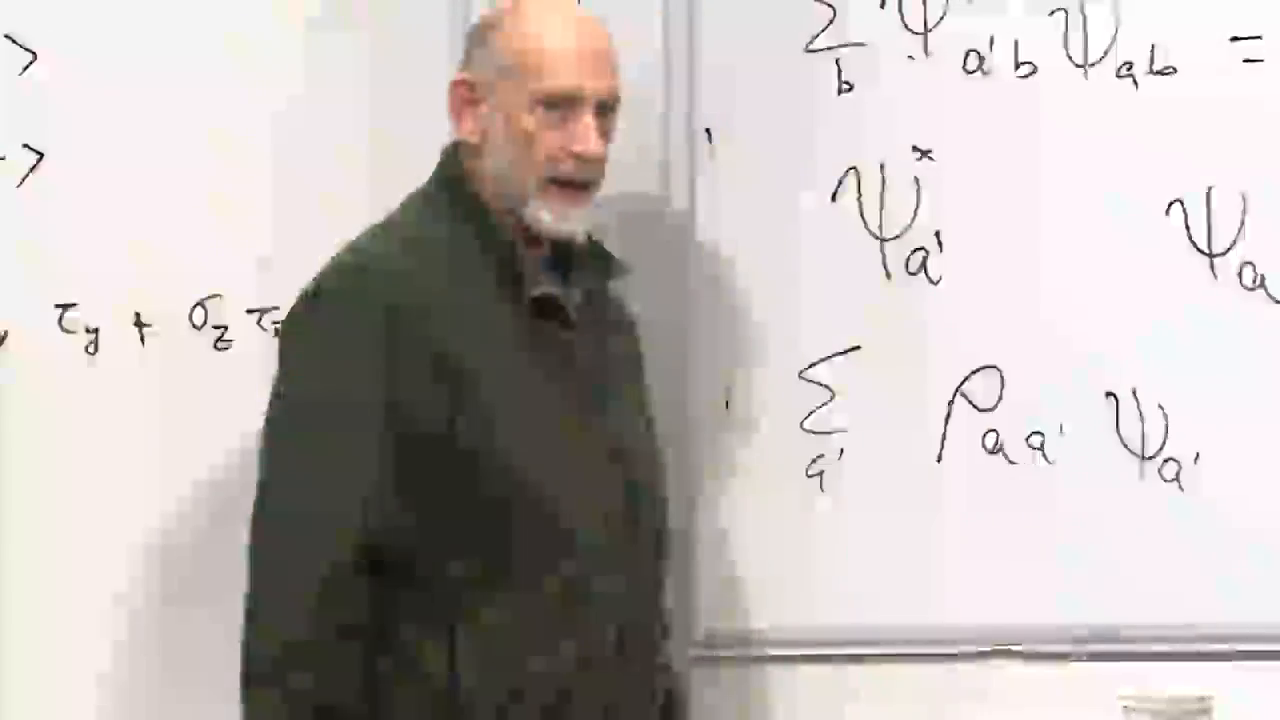
\includegraphics[width=0.88\textwidth]{lecture_07_figure_04.png}
\caption{Đối với trạng thái singlet, mỗi giá trị trung bình spin địa phương đều triệt tiêu, trong khi các thành phần bằng nhau có tích \(-1\).}
\lectureframe{00:38:28}
\end{figure}

Đây là sự đảo ngược đặc trưng do vướng víu tạo ra. Đối với một spin cô lập ở trạng thái thuần túy, luôn có một hướng mà theo đó spin của nó là xác định. Trong trạng thái singlet, không có hướng nào làm cho một trong hai spin địa phương trở nên xác định. Tuy nhiên, trạng thái hợp thành lại là thuần túy và được xác định hoàn toàn. Ta biết nhiều nhất mức mà cơ học lượng tử cho phép về toàn bộ, mà vẫn không thể gán một trạng thái thuần túy cho bất kỳ phần nào.

\begin{classroomqa}
\audiencequestion{Nếu trạng thái của toàn bộ được biết chính xác, vì sao ta không thể suy ra một trạng thái xác định cho từng spin?}
\lecturerresponse{Bởi vì trạng thái singlet không phải là trạng thái tích. Các hệ số của nó không tách thành một biên độ của Bob nhân với một biên độ của Alice. Thông tin nằm trong các quan hệ giữa các phần, chứ không nằm trong hai hàm sóng địa phương tồn tại độc lập.}
\end{classroomqa}

\begin{classroomqa}
\audiencequestion{Một toán tử như \(\sigma_z\) tự nó có thể là một trạng thái khả dĩ của spin không?}
\lecturerresponse{Không. Một trạng thái là một vectơ hoặc, tổng quát hơn, một toán tử mật độ; \(\sigma_z\) là một đại lượng quan sát tác dụng lên các trạng thái. Một vectơ riêng của \(\sigma_z\) là một trạng thái có thành phần \(z\) xác định, nhưng đại lượng quan sát và các vectơ riêng của nó là những loại đối tượng khác nhau.}
\end{classroomqa}

\begin{classroomqa}
\audiencequestion{Khi ta viết \(\sigma_z\tau_z\ket{S}=-\ket{S}\), có phải ta đã thực hiện một phép đo không?}
\lecturerresponse{Không. Phương trình ấy ghi lại cách một toán tử tác dụng lên một vectơ. Nó cho biết rằng một phép đo của đại lượng quan sát chung tương ứng chắc chắn sẽ trả về \(-1\), nhưng không có bộ dò nào được đưa vào chỉ nhờ việc viết phương trình trị riêng.}
\end{classroomqa}

\begin{classroomqa}
\audiencequestion{Một cặp vướng víu có thể chỉ tương quan một phần thôi không?}
\lecturerresponse{Có. Phản tương quan hoàn hảo là tính chất đặc biệt của trạng thái singlet đối với các trục bằng nhau. Các trạng thái vướng víu khác có thể có tương quan yếu hơn, và ngay cả trạng thái singlet cũng cho \(-\mathbf a\cdot\mathbf b\) chứ không phải \(-1\) khi hai trục khác nhau. Vướng víu liên quan đến tính không phân tích thành thừa số, chứ không phải sự trùng khớp hay trái ngược hoàn hảo trong mọi phép đo được chọn.}
\end{classroomqa}

\section{Chuẩn bị trạng thái singlet nhờ thư giãn năng lượng}

Toán tử hai spin bất biến quay
\begin{equation}
\boldsymbol{\sigma}\cdot\boldsymbol{\tau}
=\sigma_x\tau_x+\sigma_y\tau_y+\sigma_z\tau_z
\label{eq:l7-spin-dot-spin}
\end{equation}
phân tách không gian trạng thái bốn chiều. Trên trạng thái singlet,
\begin{equation}
(\boldsymbol{\sigma}\cdot\boldsymbol{\tau})\ket{S}
=-3\ket{S},
\label{eq:l7-singlet-dot-eigenvalue}
\end{equation}
còn mỗi một trong ba trạng thái triplet có trị riêng \(+1\).

\begin{figure}[htbp]
\centering
\includegraphics[width=0.88\textwidth]{lecture_07_figure_05.png}
\caption{Liên kết bất biến quay \(\boldsymbol{\sigma}\cdot\boldsymbol{\tau}\) và vai trò của nó trong việc tách riêng các phân khu singlet và triplet.}
\lectureframe{00:52:33}
\end{figure}

Giả sử Hamiltonian tương tác có chứa
\begin{equation}
H_{\mathrm{int}}
=J\,\boldsymbol{\sigma}\cdot\boldsymbol{\tau}.
\label{eq:l7-exchange-hamiltonian}
\end{equation}
Đối với liên kết phản sắt từ \(J>0\), trạng thái singlet nằm thấp hơn triplet một lượng
\begin{equation}
\Delta E=4J.
\end{equation}
Đưa hai spin lại gần nhau, cho phép các thành phần năng lượng cao hơn phân rã bằng cách phát ra một photon, một phonon hoặc một kích thích nào khác, và cặp hạt sẽ thư giãn về singlet. Sau đó có thể tách hai spin ra mà vẫn bảo toàn trạng thái chung của chúng, miễn là việc tách không đưa vào các phép quay spin mất kiểm soát hoặc làm đóng khe năng lượng quá đột ngột.

Cùng một logic năng lượng cũng xuất hiện trong các hệ nguyên tử. Chẳng hạn, trong positronium, liên kết spin giữa electron và positron làm tách các cấu hình singlet và triplet. Chênh lệch năng lượng cũng là chênh lệch khối lượng theo \(E=mc^2\), dù quang phổ học thường biểu diễn độ tách này dưới dạng năng lượng hoặc tần số.

\begin{classroomqa}
\audiencequestion{Liệu singlet có luôn là trạng thái cơ bản của hai spin tương tác không?}
\lecturerresponse{Không. Nó là trạng thái cơ bản với dấu \(J>0\) trong Phương trình~\eqref{eq:l7-exchange-hamiltonian}. Đảo dấu sẽ làm triplet thấp hơn. Lập luận chuẩn bị trạng thái phụ thuộc vào tương tác thực sự và thứ tự năng lượng của nó, chứ không chỉ đơn thuần vào sự tồn tại của hai spin.}
\end{classroomqa}

\begin{classroomqa}
\audiencequestion{Có thể đo \(\boldsymbol{\sigma}\cdot\boldsymbol{\tau}\) bằng cách đo riêng rẽ cả ba thành phần không?}
\lecturerresponse{Không thể trên một cặp duy nhất bằng ba phép đo spin cục bộ đồng thời: \(\sigma_x,\sigma_y,\sigma_z\) không tương thích với nhau, và ba thành phần của \(\tau\) cũng vậy. Giá trị kỳ vọng của nó có thể được tái dựng từ ba tập con được đo dọc theo \(x,y,z\), hoặc có thể đo trực tiếp đại lượng quan sát singlet--triplet bằng một thiết bị chung thích hợp.}
\end{classroomqa}

\begin{classroomqa}
\audiencequestion{Sau khi các spin tách ra, chúng có phải tiếp tục tương tác để vẫn vướng víu không?}
\lecturerresponse{Không. Tương tác là cần thiết để chuẩn bị hoặc làm biến đổi trạng thái, nhưng một khi singlet đã được chuẩn bị, tiến hóa đơn vị có thể bảo toàn sự vướng víu của nó mà không cần một lực tiếp diễn giữa các hạt. Từ trường cục bộ có thể quay hai thừa số, nhưng bản thân các phép quay đơn vị cục bộ không phá hủy sự vướng víu.}
\end{classroomqa}

\section{Ma trận mật độ rút gọn}

Xét lại giá trị kỳ vọng cục bộ của Alice:
\begin{equation}
\expect{L_A}
=\sum_{a',a,b}
\Psi^*(a',b)L_{a'a}\Psi(a,b).
\end{equation}
Gom lại các thừa số không thuộc về \(L\):
\begin{equation}
\expect{L_A}
=\sum_{a',a}
\left[
\sum_b\Psi(a,b)\Psi^*(a',b)
\right]L_{a'a}.
\label{eq:l7-regrouped-expectation}
\end{equation}
Biểu thức trong ngoặc vuông là ma trận mật độ rút gọn của Alice,
\begin{equation}
(\rho_A)_{aa'}
=\sum_b\Psi(a,b)\Psi^*(a',b).
\label{eq:l7-reduced-density-components}
\end{equation}
Trong ký hiệu không phụ thuộc cơ sở,
\begin{equation}
\rho_A
=\operatorname{Tr}_B\ket{\Psi}\bra{\Psi},
\label{eq:l7-partial-trace}
\end{equation}
và mọi giá trị kỳ vọng cục bộ trên phía Alice đều là
\begin{equation}
\expect{L_A}
=\operatorname{Tr}_A(\rho_A L).
\label{eq:l7-density-expectation}
\end{equation}

\begin{figure}[htbp]
\centering
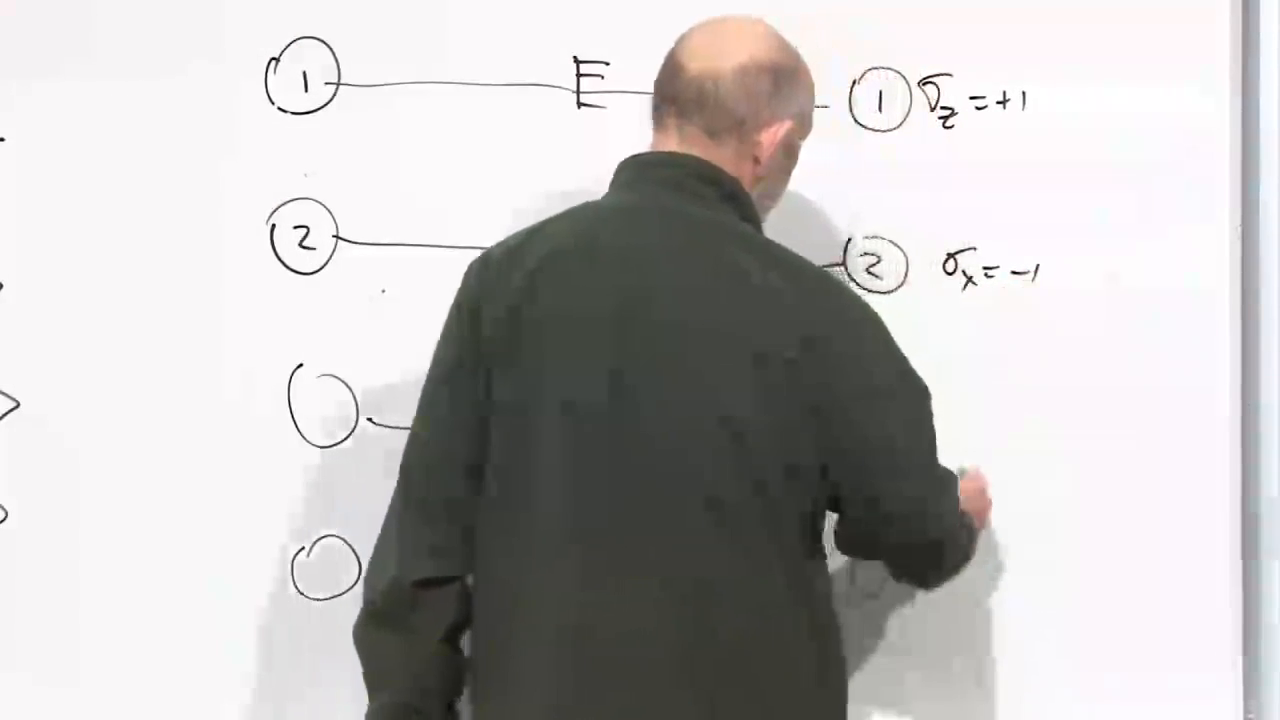
\includegraphics[width=0.88\textwidth]{lecture_07_figure_06.png}
\caption{Ma trận mật độ của Alice thu được bằng cách cộng các biên độ chung theo nhãn cơ sở của Bob.}
\lectureframe{01:02:33}
\end{figure}

Ma trận mật độ rút gọn là Hermite, dương và được chuẩn hóa:
\begin{equation}
\rho_A^\dagger=\rho_A,
\qquad
\bra{\chi}\rho_A\ket{\chi}\geq0,
\qquad
\operatorname{Tr}\rho_A=1.
\label{eq:l7-density-properties}
\end{equation}
Nó chứa đúng lượng thông tin cần thiết cho mọi phép đo chỉ giới hạn ở Alice. Nếu hai trạng thái toàn cục cho cùng \(\rho_A\), thì không thí nghiệm nào chỉ trên phía Alice có thể phân biệt chúng.

\begin{classroomqa}
\audiencequestion{Alice có đo ma trận mật độ như một đại lượng quan sát duy nhất không?}
\lecturerresponse{Không phải trong một lần đo duy nhất. Ma trận mật độ là đối tượng dùng để tính mọi xác suất đo cục bộ. Với nhiều hệ được chuẩn bị giống hệt nhau, Alice có thể tái dựng nó bằng phép chụp cắt lớp: cô ấy đo một tập đủ các đại lượng quan sát và suy ra ma trận từ các giá trị kỳ vọng của chúng.}
\end{classroomqa}

\begin{classroomqa}
\audiencequestion{Tại sao lại lấy tổng trên Bob thay vì chọn một trong các trạng thái của Bob?}
\lecturerresponse{Vì Alice không có thông tin về kết quả từ Bob. Phép vết riêng lấy tổng trên một cơ sở đầy đủ của Bob và cho trạng thái cục bộ vô điều kiện. Nếu thay vào đó chọn một kết quả của Bob, ta sẽ thu được một trạng thái có điều kiện, vốn là một phép toán khác và đòi hỏi phải biết kết quả ấy.}
\end{classroomqa}

Đối với một trạng thái tích \(\Psi(a,b)=\psi_A(a)\phi_B(b)\),
\begin{align}
(\rho_A)_{aa'}
&=\sum_b
\psi_A(a)\phi_B(b)
\psi_A^*(a')\phi_B^*(b) \\
&=\psi_A(a)\psi_A^*(a')
\sum_b|\phi_B(b)|^2 \\
&=\psi_A(a)\psi_A^*(a').
\end{align}
Do đó
\begin{equation}
\rho_A=\ket{\psi_A}\bra{\psi_A}.
\label{eq:l7-pure-projector}
\end{equation}
Đây là một phép chiếu hạng một. Tác dụng lên \(\ket{\psi_A}\) cho
\begin{equation}
\rho_A\ket{\psi_A}
=\ket{\psi_A}\braket{\psi_A}{\psi_A}
=\ket{\psi_A},
\label{eq:l7-density-on-state}
\end{equation}
Còn với mọi \(\ket{\chi}\) trực giao với \(\ket{\psi_A}\),
\begin{equation}
\rho_A\ket{\chi}
=\ket{\psi_A}\braket{\psi_A}{\chi}
=0.
\label{eq:l7-density-on-orthogonal}
\end{equation}

\begin{figure}[htbp]
\centering
\includegraphics[width=0.88\textwidth]{lecture_07_figure_07.png}
\caption{Ma trận mật độ của một trạng thái tích hoạt động như một phép chiếu: trị riêng \(1\) theo phương \(\ket{\psi_A}\) và \(0\) trên các vectơ trực giao.}
\lectureframe{01:09:43}
\end{figure}

\section{Phổ của ma trận mật độ và vướng víu}

Các trị riêng của \(\rho_A\) là không âm và có tổng bằng một. Đối với trạng thái thuần của toàn hệ:
\begin{itemize}
\item có đúng một trị riêng khác không, bằng \(1\), nghĩa là đó là trạng thái tích;
\item có hơn một trị riêng khác không nghĩa là trạng thái bị vướng víu;
\item các trị riêng bằng nhau trên toàn bộ không gian đỡ cục bộ khả dụng tương ứng với vướng víu cực đại.
\end{itemize}
Mệnh đề này thấy rõ nhất qua phân rã Schmidt,
\begin{equation}
\begin{aligned}
\ket{\Psi}_{AB}
&=\sum_{r=1}^{R}\sqrt{\lambda_r}
\ket{r}_A\ket{r}_B,\\
\lambda_r&\geq0,
\qquad
\sum_r\lambda_r=1.
\end{aligned}
\label{eq:l7-schmidt}
\end{equation}
đối với đó
\begin{equation}
\rho_A=\sum_{r=1}^{R}\lambda_r\ket{r}_A\bra{r}.
\label{eq:l7-schmidt-density}
\end{equation}
Hạng Schmidt \(R\) bằng một đối với trạng thái tích và lớn hơn một đối với trạng thái thuần vướng víu.

Đối với singlet,
\begin{equation}
\rho_A
=\operatorname{Tr}_B\ket{S}\bra{S}
=\frac12\ket{u}\bra{u}
+\frac12\ket{d}\bra{d}
=\frac12 I.
\label{eq:l7-singlet-reduced-density}
\end{equation}
Các trị riêng của nó là
\begin{equation}
\operatorname{spec}(\rho_A)
=\left\{\frac12,\frac12\right\}.
\end{equation}
Trạng thái cục bộ của Alice là hỗn hợp tối đa mặc dù trạng thái của cặp là thuần.

Phổ gợi ý một thước đo định lượng. Entropi von Neumann
\begin{equation}
S(\rho_A)
=-\operatorname{Tr}(\rho_A\log\rho_A)
=-\sum_r\lambda_r\log\lambda_r
\label{eq:l7-entanglement-entropy}
\end{equation}
bằng không đối với một trạng thái thuần tích và đạt tới \(\log d_A\) đối với một trạng thái vướng víu cực đại khi \(d_A\leq d_B\). Có thể để dành việc sử dụng chi tiết của entropy cho sau; bản thân phổ đã cung cấp sự phân biệt cốt yếu.

\begin{classroomqa}
\audiencequestion{Mọi trị riêng của một ma trận mật độ rút gọn vướng víu có nhất thiết đều khác không không?}
\lecturerresponse{Không. Có hơn một trị riêng khác không là đủ. Nếu không gian của Alice lớn, một trạng thái vướng víu có thể chỉ chiếm một không gian con Schmidt có số chiều thấp hơn, để lại thêm các trị riêng bằng không. Vướng víu cực đại nghĩa là các trị riêng bằng nhau trên toàn bộ phân hệ nhỏ hơn, chứ không chỉ là sự bằng nhau giữa một tập con được chọn tùy ý.}
\end{classroomqa}

\begin{classroomqa}
\audiencequestion{Tự bản thân một ma trận mật độ rút gọn hỗn hợp có chứng tỏ rằng Alice vướng víu với Bob không?}
\lecturerresponse{Chỉ khi biết rằng trạng thái toàn cục là thuần. Một trạng thái cục bộ hỗn hợp cũng có thể phát sinh từ một hỗn hợp cổ điển thông thường trong một trạng thái toàn cục hỗn hợp. Tuy nhiên, đối với trạng thái thuần lưỡng phần, tính hỗn hợp cục bộ là tương đương chính xác với sự vướng víu qua phép phân hoạch lưỡng phân.}
\end{classroomqa}

\begin{classroomqa}
\audiencequestion{Liệu tất cả các mômen của các đại lượng quan sát của Alice có thể xác định các phân bố xác suất của cô ấy không?}
\lecturerresponse{Trong một hệ hữu hạn chiều, các giá trị kỳ vọng của một cơ sở toán tử xác định \(\rho_A\), và \(\rho_A\) xác định mọi phân bố kết quả cục bộ thông qua quy tắc Born. Việc tái dựng đòi hỏi một ensemble gồm nhiều bản sao được chuẩn bị giống hệt nhau; một sự kiện đơn lẻ cô lập không thể cho biết một ma trận mật độ.}
\end{classroomqa}

\section{Phép đo như một tương tác gây vướng víu}

Hãy thay Alice và Bob bằng một spin và một thiết bị đo. Cho thiết bị có trạng thái sẵn sàng \(\ket{0}_D\) và trạng thái đã kích hoạt \(\ket{1}_D\). Một tương tác lý tưởng ghi lại việc spin có hướng lên hay không có thể được biểu diễn bởi
\begin{align}
\ket{u}\ket{0}_D&\longrightarrow\ket{u}\ket{1}_D,\\
\ket{d}\ket{0}_D&\longrightarrow\ket{d}\ket{0}_D.
\label{eq:l7-measurement-basis-map}
\end{align}
Bộ dò phải bắt đầu ở một trạng thái sẵn sàng đã biết; nếu không, trạng thái cuối của nó sẽ không cung cấp một bản ghi rõ ràng.

Tính tuyến tính xác định tiến hóa của một chồng chập:
\begin{equation}
\left(\alpha\ket{u}+\beta\ket{d}\right)\ket{0}_D
\longrightarrow
\alpha\ket{u}\ket{1}_D
+\beta\ket{d}\ket{0}_D.
\label{eq:l7-measurement-entanglement}
\end{equation}
Trừ khi một hệ số triệt tiêu, trạng thái cuối là vướng víu. Thiết bị đã thu nhận thông tin chính là vì trạng thái con trỏ của nó tương quan với spin.

\begin{figure}[htbp]
\centering
\includegraphics[width=0.88\textwidth]{lecture_07_figure_08.png}
\caption{Một phép đo lý tưởng tương quan các khả năng spin với các trạng thái con trỏ phân biệt và do đó tạo ra sự vướng víu.}
\lectureframe{01:20:20}
\end{figure}

Nếu chỉ giữ lại spin và bỏ qua bộ dò, trạng thái rút gọn của nó là
\begin{equation}
\rho_{\mathrm{spin}}
=|\alpha|^2\ket{u}\bra{u}
+|\beta|^2\ket{d}\bra{d},
\label{eq:l7-postmeasurement-reduced-state}
\end{equation}
giả sử các bản ghi con trỏ trực giao. Các hạng giao thoa đã biến mất khỏi mô tả cục bộ vì chúng được lưu trong các tương quan với thiết bị.

Bây giờ có hai mô tả bổ sung cho nhau. Nếu kết quả của bộ dò được đọc ra và ta điều kiện hóa theo bản ghi ấy, spin được gán cho nhánh tương ứng: \(\ket{u}\) sau khi có kích hoạt hoặc \(\ket{d}\) sau khi không có kích hoạt. Đây là mô tả sụp đổ. Nếu bộ dò và spin được xem là một hệ kín, thì Phương trình~\eqref{eq:l7-measurement-entanglement} là tiến hóa đơn vị thông thường và không nhánh nào đã bị loại khỏi trạng thái chung.

\begin{classroomqa}
\audiencequestion{Phép đo có phải là điều gì đó vượt ra ngoài sự vướng víu không?}
\lecturerresponse{Ở mức động lực học hệ--thiết bị, phép đo là một tương tác thiết lập một tương quan đáng tin cậy. Sự sụp đổ là mô tả có điều kiện được dùng sau khi một bản ghi xác định được chọn ra. Việc xem cập nhật đó là cơ bản hay là tương đối với một đường cắt được chọn là một câu hỏi diễn giải; các dự đoán thao tác là như nhau.}
\end{classroomqa}

\begin{classroomqa}
\audiencequestion{Tại sao một phép đo lý tưởng lại để nguyên trạng thái riêng của spin?}
\lecturerresponse{Đó là yêu cầu về tính lặp lại của mô hình này. Nếu đầu vào đã là một trạng thái riêng của đại lượng quan sát được đo, thì thiết bị phải ghi lại giá trị của nó mà không làm thay đổi giá trị ấy. Các phép đo thực có thể mang tính phá hủy, nhưng khi đó tương tác của chúng phải được mô hình hóa theo cách khác.}
\end{classroomqa}

\section{Thứ bậc các quan sát viên}

Một khi thiết bị đã được thừa nhận là một hệ lượng tử, thì không có lý do tự nhiên nào để dừng ở đó. Ánh sáng từ con trỏ tương tác với một con mắt; các tín hiệu từ mắt trở nên tương quan với một bộ não; một quan sát viên có thể được một quan sát viên khác quan sát. Con mèo của Schr\"odinger và người bạn của Wigner làm nổi bật cùng một cấu trúc lồng nhau:
\begin{equation}
\begin{gathered}
\text{spin}
\longrightarrow
\text{apparatus}
\longrightarrow
\text{cat}\\
\longrightarrow
\text{Schr\"odinger}
\longrightarrow
\text{Wigner}.
\end{gathered}
\label{eq:l7-observer-chain}
\end{equation}
Bên trong bất kỳ ranh giới nào được chọn, ta có thể mô tả chuỗi này bằng tiến hóa đơn vị và sự vướng víu tăng dần. Bên ngoài ranh giới ấy, ta dùng ngôn ngữ sụp đổ có điều kiện theo kết quả.

Điều kiện nhất quán then chốt là ranh giới đó có thể được dời đi. Nếu con mèo ghi nhận spin hướng lên, thì Schr\"odinger về sau cũng phải ghi nhận một con mèo đã thấy spin hướng lên, và Wigner phải ghi nhận Schr\"odinger ghi nhận cùng lịch sử đó. Cơ học lượng tử không chỉ ra một đường ranh sắc nét duy nhất mà tại đó bắt buộc phải tuyên bố một sự kiện khách quan. Con mèo, mắt và não đều được tạo thành từ các bậc tự do vật lý; miễn trừ một trong số chúng khỏi cơ học lượng tử sẽ đòi hỏi một định luật bổ sung.

Thái độ của Feynman trước sự bất an nảy sinh từ đó là thực dụng. Vấn đề khái niệm có thể lớn đến mức khó thậm chí nói rõ liệu thực sự có một vấn đề như vậy hay không, trong khi các quy tắc tính toán vẫn tiếp tục cho tiên đoán đối với mọi thí nghiệm trong phạm vi áp dụng của chúng. Mục đích của hình thức luận không phải là ép buộc một cách diễn giải duy nhất, mà là làm cho nguồn gốc của sự bất an ấy trở nên chính xác: tri thức đầy đủ về một toàn thể có thể cùng tồn tại với việc không có bất kỳ mô tả trạng thái thuần nào cho các bộ phận của nó.

\begin{classroomqa}
\audiencequestion{Nếu tôi là con mèo, tôi có phải vạch đường ranh ở chính mình không?}
\lecturerresponse{Bạn có thể dùng mô tả sụp đổ cho bản ghi xác định sẵn có đối với mình. Một quan sát viên khác, người bao gồm bạn trong một hệ cô lập lớn hơn, có thể dùng mô tả trạng thái vướng víu. Điều được đòi hỏi không phải là mọi người vạch cùng một đường ranh, mà là mọi mô tả phải cho các bản ghi nhất quán bất cứ khi nào các quan sát viên về sau đối chiếu kết quả.}
\end{classroomqa}

\begin{classroomqa}
\audiencequestion{Sự kiện khách quan xảy ra ở đâu: tại nguyên tử, con mèo, Schr\"odinger, hay Wigner?}
\lecturerresponse{Hình thức luận đơn vị không chọn một vị trí nào trong số đó làm ranh giới đặc quyền. Có lẽ những từ thông thường như \emph{xảy ra} đang bị đẩy vượt ra ngoài ngữ cảnh mà trong đó chúng còn chính xác. Các công cụ hình thức cho ta biết các tương quan lan truyền như thế nào và mỗi quan sát viên có thể dự đoán điều gì; việc quyết định phải diễn giải ranh giới cuối cùng ra sao là một nhiệm vụ riêng.}
\end{classroomqa}

\subsection{Ghép yếu và phép đọc ra không hoàn hảo}

Ánh xạ lý tưởng trong Phương trình~\eqref{eq:l7-measurement-basis-map} tạo ra các bản ghi phân biệt hoàn toàn. Một tương tác yếu hơn có thể khiến các trạng thái của thiết bị chỉ phân biệt được một phần:
\begin{equation}
\alpha\ket{u}\ket{D_u}
+\beta\ket{d}\ket{D_d},
\qquad
0<|\braket{D_d}{D_u}|<1.
\label{eq:l7-weak-measurement}
\end{equation}
Khi đó thiết bị chỉ nhận được thông tin từng phần và sự vướng víu là không hoàn toàn. Đây là bối cảnh của một phép đo yếu hoặc không sắc.

Cần phân biệt tình huống đó với một khâu đọc ra về sau bị kém. Bộ dò có thể đã tương quan hoàn toàn với spin trong khi mắt, cáp, bộ khuếch đại hoặc não lại không truyền bản ghi một cách rõ ràng. Trong trường hợp thứ nhất, tương tác hệ--bộ dò là yếu; trong trường hợp thứ hai, một bản ghi tốt đã có ở bộ dò nhưng sự truyền thông tin về sau lại kém hiệu quả. Hiệu suất của bộ dò có thể liên quan đến một trong hai giai đoạn, vì vậy phải xác định ghép nối vật lý trước khi quy nguyên nhân.

\begin{classroomqa}
\audiencequestion{Nếu thị lực kém làm kim chỉ thị trở nên không rõ ràng, thì phép đo lượng tử có phải là yếu không?}
\lecturerresponse{Không nhất thiết. Spin có thể đã tương quan mạnh và hoàn toàn với thiết bị, trong khi kênh từ thiết bị đến mắt hoặc từ mắt đến não lại kém. Một phép đo thật sự yếu có nghĩa là chính sự ghép nối ban đầu hệ--thiết bị chỉ tạo ra các bản ghi chỉ phân biệt được một phần.}
\end{classroomqa}

\section{Tính địa phương và không truyền tín hiệu}

Cụm từ \emph{tác dụng từ xa} nên được gán một nghĩa thao tác. Trong vật lý thông thường, một tác động ở xa làm thay đổi những gì có thể quan sát được tại đây. Nếu Mặt Trời biến mất và chuyển động của Trái Đất thay đổi ngay lập tức, thay vì sau thời gian ánh sáng truyền đi, thì người ta có thể dùng sự thay đổi ấy để truyền thông tin nhanh hơn ánh sáng. Đó sẽ là sự truyền tín hiệu phi địa phương thực sự.

Sự rối không cho phép kiểu truyền tín hiệu như vậy. Giả sử Bob thực hiện một phép toán lượng tử địa phương được biểu diễn bởi các toán tử Kraus \(K_\mu\), với
\begin{equation}
\sum_\mu K_\mu^\dagger K_\mu=I_B.
\end{equation}
Nếu Alice không biết kết quả của Bob, thì trạng thái chung cuối cùng là
\begin{equation}
\rho'_{AB}
=\sum_\mu
(I_A\otimes K_\mu)\rho_{AB}
(I_A\otimes K_\mu^\dagger).
\end{equation}
Lấy vết riêng phần theo Bob, ta được
\begin{equation}
\rho'_A
=\operatorname{Tr}_B\rho'_{AB}
=\operatorname{Tr}_B\rho_{AB}
=\rho_A.
\label{eq:l7-no-signaling}
\end{equation}
Vì thế, mọi xác suất địa phương không điều kiện của Alice đều không đổi dưới lựa chọn một phép toán địa phương bảo toàn vết của Bob.

Các trạng thái có điều kiện thì khác. Nếu Bob đo và thu được kết quả \(\mu\), Alice có thể gán
\begin{equation}
\rho_{A|\mu}
=\frac{
\operatorname{Tr}_B\!\left[
(I_A\otimes K_\mu)\rho_{AB}
(I_A\otimes K_\mu^\dagger)
\right]
}{p_\mu}.
\label{eq:l7-conditioned-state}
\end{equation}
Nhưng Alice không thể biết \(\rho_{A|\mu}\) nào áp dụng cho đến khi Bob truyền \(\mu\) bằng một tín hiệu thông thường. Trước khi thông điệp đến, cô ấy phải lấy trung bình trên các kết quả:
\begin{equation}
\sum_\mu p_\mu\rho_{A|\mu}=\rho_A.
\label{eq:l7-conditioned-average}
\end{equation}

\begin{classroomqa}
\audiencequestion{Nếu Bob đo trước, thì khi nào ma trận mật độ của Alice thay đổi?}
\lecturerresponse{Ma trận mật độ không điều kiện của cô ấy không thay đổi. Khi kết quả của Bob đến được với cô ấy, cô ấy có thể thay nó bằng ma trận mật độ có điều kiện tương ứng. Sự cập nhật đó phản ánh thông tin mới trở nên sẵn có và không thể được dùng trước khi thông điệp cổ điển tới nơi.}
\end{classroomqa}

\begin{classroomqa}
\audiencequestion{Phép đo của Bob có làm sụp đổ về mặt vật lý trạng thái của Alice đúng vào cùng thời điểm không?}
\lecturerresponse{Các cách diễn giải khác nhau mô tả sự cập nhật có điều kiện theo những cách khác nhau, nhưng tất cả đều đồng ý về phát biểu có thể kiểm nghiệm được: các xác suất kết quả địa phương của Alice vẫn không đổi cho đến khi thông tin từ Bob trở nên sẵn có. Không tạo ra một tín hiệu tức thời có thể điều khiển nào.}
\end{classroomqa}

Hãy hình dung nhiều cặp singlet được phân phát thành các hàng được đánh số. Ở một thành viên, Bob đo \(z\), ở một thành viên khác \(x\), ở một thành viên khác nữa \(y\), v.v. Các kết quả địa phương của Alice vẫn là một dãy không thiên lệch trong mọi hàng:
\begin{equation}
P_A(+|\mathbf a)=P_A(-|\mathbf a)=\frac12.
\label{eq:l7-alice-marginal}
\end{equation}
Không có gì trong sổ ghi chép của cô ấy cho biết Bob đã chọn những trục nào hay đã thu được những kết quả nào.

\begin{figure}[htbp]
\centering
\includegraphics[width=0.88\textwidth]{lecture_07_figure_09.png}
\caption{Nhiều cặp được chuẩn bị độc lập cho phép gán các trục đo khác nhau cho các hàng khác nhau; thống kê biên của Alice vẫn không đổi.}
\lectureframe{01:49:00}
\end{figure}

Sau khi một bức điện tín bị giới hạn bởi tốc độ ánh sáng đến nơi, liệt kê trục và kết quả của Bob cho từng hàng, Alice có thể sắp xếp lại các bản ghi của mình. Khi ấy, các phép đo singlet theo cùng trục sẽ cho kết quả đối nhau từng cặp một. Thông điệp làm lộ ra những tương quan vốn đã có trong thống kê chung; nó không hồi tố làm thay đổi phân bố tần suất địa phương trước đó của Alice.

\begin{classroomqa}
\audiencequestion{Alice có thể suy ra lựa chọn của Bob từ đủ nhiều mômen của chính dữ liệu của mình không?}
\lecturerresponse{Không. Mọi mômen địa phương của Alice đều được cố định bởi \(\rho_A\), và theo phương trình~\eqref{eq:l7-no-signaling}, ma trận đó không đổi. Nhiều bản sao hơn chỉ cải thiện ước lượng của cô ấy về cùng một ma trận mật độ địa phương; chúng không tiết lộ cơ sở hay kết quả của Bob.}
\end{classroomqa}

\begin{classroomqa}
\audiencequestion{Nếu Bob chọn một trục khác nhau trên mỗi thành viên của tập hợp thì sao?}
\lecturerresponse{Alice vẫn thấy cùng một phân bố địa phương. Khi Bob gửi các thiết lập và kết quả theo từng hàng, hai bên có thể so sánh các tương quan có điều kiện cho từng cặp trục. Sự phụ thuộc vào thiết lập xuất hiện trong thống kê chung, không phải trong thống kê biên của Alice.}
\end{classroomqa}

\section{Câu hỏi của Bell như một trò chơi mô phỏng}

Sự phân biệt giữa không truyền tín hiệu và tính phi địa phương theo Bell trở nên rõ hơn khi xét như một bài toán mô phỏng cổ điển. Bắt đầu với một spin,
\begin{equation}
\ket{\psi}=\alpha_u\ket{u}+\alpha_d\ket{d},
\qquad
|\alpha_u|^2+|\alpha_d|^2=1.
\end{equation}
Một chương trình cổ điển có thể lưu hai biên độ phức, cho chúng tiến triển theo phương trình Schr\"odinger, và nhận một hướng đo do người dùng chọn. Khi lệnh đo được đưa ra, chương trình tính các xác suất Born, dùng một bộ sinh số giả ngẫu nhiên để chọn một kết quả, hiển thị kết quả đó, và cập nhật trạng thái đang lưu thành trạng thái riêng tương ứng. Lặp lại quá trình này sẽ tái tạo thống kê của một spin.

Vì thế, chỉ riêng tính ngẫu nhiên không phải là ranh giới phân chia giữa cơ học cổ điển và cơ học lượng tử. Máy tính cổ điển có thể tạo ra các dãy đủ ngẫu nhiên về mặt thao tác cho một mô phỏng, ngay cả khi các thuật toán giả ngẫu nhiên của chúng ở bên dưới là tất định.

Đối với hai spin ở trạng thái tích, hai máy tính tách biệt cũng đủ. Máy của Alice lưu và cho \(\ket{\psi_A}\) tiến triển; máy của Bob lưu và cho \(\ket{\phi_B}\) tiến triển. Mỗi máy chỉ phản ứng với thiết lập địa phương của riêng nó. Vì các xác suất chung phân tích thành tích, nên sau khi hai máy tách ra không cần liên lạc nào nữa.

Một cặp rối làm thay đổi bài toán. Trước thí nghiệm, ta có thể đưa hai máy lại gần nhau, nạp dữ liệu ẩn có tương quan, đồng bộ hóa đồng hồ của chúng, và thậm chí cấp cho chúng cùng một giá trị khởi tạo cho bộ sinh số ngẫu nhiên. Tuy nhiên, sau khi tách ra, mỗi đầu ra chỉ được phụ thuộc vào thiết lập đo địa phương của nó và thông tin chung đã được cung cấp từ trước. Định lý Bell cho thấy không có sơ đồ biến ẩn địa phương nào như vậy tái tạo được mọi tương quan lượng tử đối với các thiết lập được chọn tự do.

\begin{figure}[htbp]
\centering
\includegraphics[width=0.88\textwidth]{lecture_07_figure_10.png}
\caption{Mô hình hai máy tính tách biệt: các chương trình địa phương có thể chia sẻ dữ liệu chuẩn bị, nhưng sau khi tách ra chúng không thể truyền cho nhau các thiết lập đo.}
\lectureframe{02:00:00}
\end{figure}

Nếu vẫn còn dây nối giữa hai máy tính để các thiết lập và kết quả có thể được trao đổi, thì mô phỏng có thể tái tạo các tương quan. Nhưng khi đó, cặp này không còn là một mô hình địa phương tách biệt đúng nghĩa nữa; nó hoạt động như một máy tính được nối thành một khối. Trở ngại ở đây không phải là tính toán cổ điển theo nghĩa trừu tượng. Một máy cổ điển toàn cục duy nhất có thể mô phỏng các hệ lượng tử hữu hạn bằng cách lưu toàn bộ hàm sóng chung, mặc dù bộ nhớ cần thiết nói chung tăng theo hàm mũ với số phân hệ. Trở ngại của Bell liên quan đến việc phân rã thành các máy địa phương vận hành độc lập.

\begin{classroomqa}
\audiencequestion{Vì sao hai máy tính không thể đơn giản dùng cùng một dãy số ngẫu nhiên?}
\lecturerresponse{Ngẫu nhiên chung đã được cho phép sẵn trong một mô hình biến ẩn địa phương. Nó có thể ấn định trước các câu trả lời có tương quan, nhưng mỗi câu trả lời phải dùng được cho mọi thiết lập đo mà về sau có thể được chọn ở phía đó. Các bất đẳng thức Bell biểu thị những ràng buộc mà mọi chiến lược địa phương được sắp đặt từ trước như vậy đều tuân theo; các tương quan lượng tử vi phạm những ràng buộc ấy.}
\end{classroomqa}

\begin{classroomqa}
\audiencequestion{Các số ngẫu nhiên có phải phụ thuộc vào các hướng đo không?}
\lecturerresponse{Một đầu ra địa phương có thể phụ thuộc vào hướng địa phương của chính nó và dữ liệu ẩn chung, nhưng không thể phụ thuộc vào hướng ở xa được chọn sau khi đã tách ra. Cho phép phụ thuộc vào cả hai thiết lập đòi hỏi phải có liên lạc, phản nhân quả, hoặc sự thất bại của giả định độc lập đo lường thường dùng. Định lý Bell làm cho những giả định này trở nên minh nhiên thay vì che giấu chúng trong từ \emph{ngẫu nhiên}.}
\end{classroomqa}

\begin{classroomqa}
\audiencequestion{Liệu hai máy tính lượng tử tách biệt có thể thành công ở chỗ các chương trình cổ điển thất bại không?}
\lecturerresponse{Chúng có thể thành công nếu chúng chia sẻ các bậc tự do lượng tử bị rối. Trong trường hợp đó, các máy tính không mô phỏng sự rối bằng các bản ghi cổ điển địa phương; chúng sở hữu nó về mặt vật lý. Các kết quả địa phương của chúng vẫn không thể truyền một thông điệp nhanh hơn ánh sáng có thể điều khiển được.}
\end{classroomqa}

\begin{classroomqa}
\audiencequestion{Một máy tính cổ điển thông thường có thể mô phỏng toàn bộ cặp không?}
\lecturerresponse{Có. Nó có thể lưu bốn biên độ chung và tính mọi xác suất đo ở một chỗ. Đối với nhiều hạt, mô phỏng trực tiếp này trở nên tốn kém vì số chiều của không gian Hilbert tăng theo hàm mũ, nhưng không có mâu thuẫn Bell nào khi toàn bộ thông tin sẵn có một cách toàn cục bên trong một máy.}
\end{classroomqa}

\begin{classroomqa}
\audiencequestion{Vậy định lý Bell có chứng minh tác dụng từ xa theo nghĩa thông thường không?}
\lecturerresponse{Nó chứng minh rằng các lời giải thích biến ẩn địa phương thỏa mãn các giả định của Bell không thể tái tạo những tương quan được quan sát. Nó không cung cấp cho Alice hay Bob một kênh truyền tín hiệu siêu ánh sáng. Tính phi địa phương theo Bell và sự truyền thông tin nhanh hơn ánh sáng theo nghĩa thao tác là hai khẳng định khác nhau.}
\end{classroomqa}

\section{Có thể biết được gì một cách địa phương?}

Không được đánh đồng các đại lượng quan sát địa phương với các đại lượng quan sát chung. Bob có thể đo \(\sigma_x\) và Alice có thể đo \(\tau_x\); bằng cách đối chiếu các bản ghi sau đó, họ ước lượng
\begin{equation}
\expect{\sigma_x\tau_x}.
\end{equation}
Không có thiết bị địa phương nào tự nó đo được tích đó. Đại lượng vô hướng đối với phép quay
\begin{equation}
\boldsymbol{\sigma}\cdot\boldsymbol{\tau}
=\sigma_x\tau_x+\sigma_y\tau_y+\sigma_z\tau_z
\end{equation}
đòi hỏi либо các dưới-tập hợp khác nhau cho ba hạng, либо một thiết bị chung mới phân giải được các tiểu không gian singlet và triplet. Không thể thu được cả ba tích thành phần không tương thích từ một cặp bằng các máy đo spin địa phương ban đầu.

\begin{classroomqa}
\audiencequestion{Có những đại lượng quan sát của toàn hệ mà các thiết bị ban đầu của Alice và Bob không thể đo riêng rẽ hay không?}
\lecturerresponse{Có. Một tích đơn lẻ như \(\sigma_x\tau_x\) có thể được ước lượng bằng hai phép đo địa phương theo \(x\) rồi so sánh kết quả. Tổng \(\boldsymbol{\sigma}\cdot\boldsymbol{\tau}\) không thể được lắp ghép từ các số đọc đồng thời \(x,y,z\) trên một cặp. Nó cần một phép đo singlet--triplet thật sự chung hoặc các tập hợp riêng biệt cho các hạng không tương thích.}
\end{classroomqa}

Bob không thể suy ra sự rối từ một sự kiện đơn lẻ. Tuy nhiên, với nhiều bản sao được chuẩn bị giống hệt nhau, anh ấy có thể phục dựng ma trận mật độ rút gọn của mình. Đối với một qubit,
\begin{equation}
\rho_B
=\frac12\left(
I+\mathbf r\cdot\boldsymbol{\sigma}
\right),
\label{eq:l7-bloch-density}
\end{equation}
và các phép đo dọc theo nhiều trục xác định vectơ Bloch \(\mathbf r\). Nếu \(|\mathbf r|=1\), trạng thái địa phương của Bob là thuần; nếu \(|\mathbf r|<1\), nó là hỗn hợp. Trong trường hợp đặc biệt khi sự chuẩn bị toàn cục được biết là cùng một trạng thái thuần trên mọi lần thử, tính hỗn hợp địa phương chứng minh rằng Bob bị rối với một hệ nào đó bên ngoài phân hệ của mình.

Đối với tích của hai spin thuần, Bob có thể tìm hướng phân cực \(\mathbf n=\mathbf r/|\mathbf r|\). Dọc theo trục đó, các phép đo lặp lại cho một kết quả xác định. Đối với singlet, \(\mathbf r=0\), nên mọi trục vẫn ngẫu nhiên ở mức địa phương. Việc tìm kiếm ấy không bao giờ tìm thấy một hướng phân cực.

\begin{classroomqa}
\audiencequestion{Bob có thể phát hiện sự rối mà không cần nói chuyện với Alice không?}
\lecturerresponse{Từ một tập hợp, anh ấy có thể phát hiện rằng trạng thái rút gọn của riêng mình là hỗn hợp. Nếu anh ấy cũng biết rằng mọi cặp đều được chuẩn bị trong cùng một trạng thái thuần toàn cục, anh ấy có thể suy ra sự rối qua ranh giới đó. Nếu không có giả định thuần ấy, trạng thái hỗn hợp của anh ấy thay vào đó có thể bắt nguồn từ một hỗn hợp chuẩn bị cổ điển, và chỉ dữ liệu địa phương thôi sẽ không quyết định được sự phân biệt này.}
\end{classroomqa}

\begin{classroomqa}
\audiencequestion{Vì sao cần nhiều hệ được chuẩn bị giống hệt nhau?}
\lecturerresponse{Mỗi phép đo spin chỉ cho một kết quả và nói chung làm nhiễu bản sao đó. Vì vậy, phép chụp cắt lớp phân bố các phép đo không tương thích trên một tập hợp được chuẩn bị bằng cùng một quy trình. Ma trận mật độ và phổ của nó là những tính chất thống kê được suy ra từ các lần thử lặp lại đó, chứ không phải những nhãn được bộc lộ bởi một hạt đơn lẻ.}
\end{classroomqa}

Mạch lập luận giờ đây khép lại đúng tại điểm nó bắt đầu. Vướng víu lượng tử không phải là sự cùng chia sẻ một trạng thái theo nghĩa mơ hồ. Đó là tính không thể phân tích một trạng thái thuần chung thành tích, biểu hiện cục bộ qua một ma trận mật độ rút gọn không phải là toán tử chiếu, và ở mức toàn hệ qua những tương quan không thể tái tạo bằng việc ghi sổ cổ điển tách rời. Toàn thể có thể được biết hoàn toàn, trong khi mỗi phần vẫn ở trạng thái hỗn hợp. Chính sự kiện đó làm cho phép đo trở nên khả dĩ, bảo toàn nguyên lý không truyền tin, và cung cấp cấu trúc mà định lý Bell sẽ kiểm định.
